\documentclass[a4paper]{article}


\bibliographystyle{abbrv}
\usepackage{amsfonts}
\usepackage{amsthm}
\usepackage{amssymb}
\usepackage{amsmath}
\usepackage{enumerate}
\usepackage{fancyhdr}
\usepackage{mathabx}
\usepackage{verbatim}
\usepackage{tikz}

%%%%%%%%%%%%%%%%%%%%%%%%%%%%%%%%%%%%%%%%%%%%%%%%%%%%%%%
%% Setting for the nice arrows and nodes graphs  %%%%%%
%%%%%%%%%%%%%%%%%%%%%%%%%%%%%%%%%%%%%%%%%%%%%%%%%%%%%%%

\usetikzlibrary{arrows,positioning,decorations.markings} 
\tikzset{
    %Define standard arrow tip
    >=stealth',
    %Define style for boxes
    punkt/.style={
           rectangle,
           rounded corners,
           draw=black, very thick,
           text width=6.5em,
           minimum height=2em,
           text centered},
    % Define arrow style
    pil/.style={
           ->,
           thick,
           shorten <=2pt,
           shorten >=2pt,}
}
\tikzstyle{vecArrow} = [thick, decoration={markings,mark=at position
   1 with {\arrow[semithick]{open triangle 60}}},
   double distance=1.4pt, shorten >= 5.5pt,
   preaction = {decorate},
   postaction = {draw,line width=1.4pt, white,shorten >= 4.5pt}]
\tikzstyle{innerWhite} = [semithick, white,line width=1.4pt, shorten >= 4.5pt]

%%%%%%%%%%%%%%%%%%%%%%%%%%%%%%%%%%%%%%%%%%%%%%%%%%%%%%%%
%%%%%%%%%%%%%%%%%%%%%%%%%%%%%%%%%%%%%%%%%%%%%%%%%%%%%%%%

\usepackage[all]{xy}

% \usepackage{showlabels}
%  Formatting matters
% original dimensions

\textwidth=5.75truein
\textheight=8.5truein


% dimensions to play with
%\textheight=8.0truein   %for mac
%\textwidth=6.0truein

\oddsidemargin=0.3truein
\evensidemargin=0.3truein

%\topmargin=-0.35truein %original
\topmargin=-0.25truein
% \headheight=0.16truein
\headheight=13pt
\headsep=0.3truein

\footskip=0.5truein

\parindent=18pt
\tolerance=6000
\parskip=0pt
\linespread{1.02}

\newcommand{\N}{\mathbb{N}}
\newcommand{\Z}{\mathbb{Z}}
\newcommand{\R}{\mathbb{R}}
\newcommand{\Q}{\mathbb{Q}}
\newcommand{\C}{\mathbb{C}}
\newcommand{\T}{\mathbb{T}}
\newcommand{\h}{\mathcal{H}}
\newcommand{\Manoa}{M\=anoa}
\newcommand{\Hawaii}{Hawai\kern.05em`\kern.05em\relax i}
\theoremstyle{plain}
\newtheorem{theorem}{Theorem}[section]
\newtheorem{lemma}[theorem]{Lemma}
\newtheorem{corollary}[theorem]{Corollary}
\newtheorem{proposition}[theorem]{Proposition}
\newtheorem{conjecture}[theorem]{Conjecture}
\newtheorem{definition-theorem}[theorem]{Definition / Theorem}
\newtheorem{project}[theorem]{Project}

% without a number

\newtheorem*{conjecture*}{Conjecture}
\newtheorem*{theorem*}{Theorem}
\theoremstyle{definition}
\newtheorem{definition}[theorem]{Definition}
\newtheorem{example}[theorem]{Example}
\newtheorem{notation}[theorem]{Notation}
\newtheorem{convention}[theorem]{Convention}
\theoremstyle{remark}
\newtheorem{remark}[theorem]{Remark}
\newtheorem{remarks}[theorem]{Remarks}

% without a number

\newtheorem*{example*}{Example}  
\newtheorem*{remark*}{Remark}


\geometry{hmargin=2.5cm,vmargin=1.5cm}

\title{Research project}
% and PhD description}

\date{}
\author{ Cl\'ement Dell'Aiera}


%\usepackage{fullpage}

\begin{document}

\maketitle
%\newpage
%\tableofcontents
This document describes the future directions that I will be trying to study in the next years. I am also interested in any other project which would lead to fruitful collaborations. The piece is divided into two parts: a general introduction focusing on ideas and motivations for my main field of study, followed by a succession of research projects and questions, oriented towards a reader more aware of Operator Algebras and Noncommutative Geometry. 
%the work done under the supervision of Hervé Oyono-Oyono during my PhD thesis in Metz, at the Elie Cartan’s Institute of Lorraine.
%, and then presents my research project. 
%I am currently a graduate student at the University of Lorraine, and I am beginning my third year of PhD. I am supposed to defend my PhD thesis before June 2017. My work should be submitted within several weeks, and I am very happy to send the preprint version of my work to anyone who is interested in having more details. \\

\section{General introduction}

This section describes several research projects that we submit for the proposal for the next three years. We organized these into two sections entitled \textit{Weak decompositions} and \textit{Quantum groups}. Before this, we first give some background. The author will try to explain how the current questions in \textit{Operator Algebras} and \textit{Noncommutative Geometry} they are interested in are related to other parts of mathematics. Our point of view is to see our activity as an offspring of Grothendieck's work on tensor products of Banach spaces.    

\subsection{From approximation properties to the K\"unneth formula in operator $K$-theory and the Universal Coefficient Theorem}

An important part of Operator Algebras as a field can be described as attempting to answer questions arising in Functional Analysis using other seemingly unrelated fields, the most common being Topological Dynamics, Group and Geometric Group theory. A good starting point to understand these preocupations is the work of Alexander Grothendieck on tensor products of topological vector spaces. \\

At the time, starting his PhD in Nancy, Grothendieck was asked by Laurent Schwartz to develop a theory of tensor products for topological vector spaces. This question was motivated by the kernel theorem, whose proof was found to be too involved by Laurent Schwartz in the general case, whereas the finite dimensional case reduces to the fact that 
\[V^*\otimes W \cong Hom(V,W),\] 
where $V$ and $W$ are finite dimensional vector spaces and $Hom(V,W)$ is the space of linear maps $V\rightarrow W$. Having topological tensor products in one's toolbox led to hope for a simpler and more natural proof. The rest of the story is well known: Grothendieck found that one could define a lot of completions of the algebraic tensor products. Spaces admitting only one such completion were called \textit{nucl\'eaires}, or nuclear, after the kernel theorem (\textit{nucl\'eaires} means ``related to the kernel" in French).\\

The paper \textit{R\'esum\'e de la th\'eorie m\'etrique des produits tensoriels topologiques} \cite{GrothendieckResume}, commonly know as the Resum\'e, enhanced a vast research program. It specialized the work to the case of Banach spaces. Surprisingly, the paper did not attract a lot of attention at the time of its publication, maybe because the trend was back then to focus on locally convex spaces. The paper was rediscovered fifteen years later. See Pisier's paper \cite{PisierSurvey} for a very nice survey on the subject.\\

Approximation theory for $C^*$-algebras is a direct offspring of this work. The idea is to study properties of various constructions such as tensor products or crossed-products (which is a twisted version of tensor products) of $C^*$-algebras. It is very useful in that case to use spaces of functions on a topological group as a tool to construct exotic examples. Let me illustrate this by the following example.\\

John Von Neumann defined a property on groups called \textit{amenability} as follows. A discrete countable group $\Gamma$ is said to be amenable if there exists an invariant mean (i.e. $\Gamma$-invariant linear positive functional) $m: l^\infty(\Gamma)\rightarrow \C$. Now, the group ring $\C[\Gamma]$ is a $*$-algebra w.r.t. the convolution as a product and $(z. \gamma)^* = \overline{z}\gamma^{-1}$. This algebra can be represented as a self adjoint subalgebra of the bounded operators on the complex Hilbert space $l^2\Gamma$ by what is called the left regular representation $\lambda_\Gamma: \C[\Gamma]\rightarrow B(l^2\Gamma)$. The reduced $C^*$-algebra of the group $\Gamma$ is defined as the closure of the image of the regular representation.\\

It turns out that, for such a group $\Gamma$, this $C^*$-algebra is nuclear iff $\Gamma$ is amenable. Thus, examples of nonamenable groups (like any nonabelian free group) provide instances of nonnuclear $C^*$-algebras. This example is typical of how a completely group theoretic property can be used to provide contructions of Banach algebras with interesting properties. Many other areas of mathematics contribute to fuel new ideas in operator algebras. A nice object which is general enough to encompass all of these constructions and provides easily a $C^*$-algebra is a \textit{groupoid}. For our purpose, the reader only needs to know that a groupoid is meant to be two locally compact spaces: the objects $G^0$ and the arrows $G$. $G$ is ``group like" in the sense that it has a partial multiplication law and every arrow has an inverse for it. The difference with a group is that $G$ sits over the base space $G^0$: every arrow has a source and a target in $G^0$.\\  

This extra flexibility makes groupoids very versatile. Indeed, out of an action by homeomorphisms of a group $\Gamma$ on a topological space $\Omega$ or out of a metric space $X$, one can build groupoids (respectively the action groupoid $\Omega \rtimes \Gamma$ and the coarse groupoid $G(X)$ \cite{SkTuYu}) nice enough to have convolution algebras. \\  
%Amenability was of uttermost importance in the classification of factors obtained by Connes \cite{}. \\ 

% Examples from http://www.texample.net/tikz/examples/borrowers-and-lenders/ 
% and http://www.texample.net/tikz/examples/double-arrows/

%%%%%%%%%%%%%%%%%%%%%%%%%%%%%%%%%%%%%%%%%%%%%%%%%%%%%%%%%%%%%%%%%%%%%%%%%%%
\[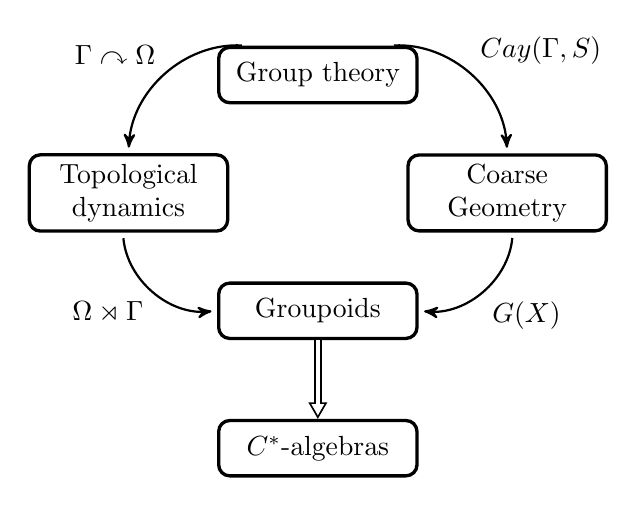
\begin{tikzpicture}[node distance=1cm, auto,]
 %nodes
\node[punkt] (C) {$C^*$-algebras};\\
\node[punkt, above=of C] (G) {Groupoids};
\node[above=of G] (dummy) {};
\node[punkt, right=of dummy] (CG) {Coarse Geometry}
	edge[pil, bend left=45] node[auto] {$G(X)$} (G.east); 
\node[punkt, left=of dummy] (TD) {Topological dynamics}
	edge[pil, bend right=45] node[auto] [below left] {$\Omega\rtimes \Gamma$} (G.west); 
\node[punkt, above=of dummy] (GT) {Group theory}
	edge[pil, bend left=45] node[auto] {$Cay(\Gamma,S)$} (CG.north) 
	edge[pil, bend right=45] node[auto] [above left] {$\Gamma \curvearrowright \Omega$} (TD.north);

\draw[vecArrow] (G) to (C);
\end{tikzpicture}\]
%%%%%%%%%%%%%%%%%%%%%%%%%%%%%%%%%%%%%%%%%%%%%%%%%%%%%%%%%%%%%%%%%%%%%%%%%%%

Taking a property in any of these areas, trying to define it in the setting of groupoids, then unravelling the definition in another setting has proven to be a very fruitful strategy. For instance, amenability can be easily defined for locally compact groupoids \cite{anantharaman2000amenable}. But if one looks at the coarse groupoid $G(X)$ of a metric space, saying it is amenable is equivalent to say that $X$ has Yu's property (A) (a \textit{coarse} version of amenability). Another direction is to use properties of groupoids to build interesting classes of $C^*$-algebras. For instance, second countable locally compact amenable groupoids have reduced $C^*$-algebras that are known to satisfy the K\"unneth formula. \\

Over the years, other properties have been found to be of interest. Without pretending to be exhaustive, let us just mention exactness, simplicity, finite nuclear dimension, the UCT class, the Bootstrap class,... Usually these classes are important because of their relation to Elliot's classification program, or to topology and geometry. \\

One of the objects of importance for $C^*$-algebras are the \textit{operator $K$-theory groups} $K_0(A)$ and $K_1(A)$, which are homotopy invariant abelian groups associated to any $C^*$-algebras. Let us just say that $K_0(A)$ is built out of equivalence classes of projections in $M_n(A)$, while $K_1(A)$ is built from equivalence classes of unitaries in $M_n(A)$. These groups are a generalized cohomology theory on the category of $C^*$-algebras. Georges Elliott suggested that all separable nuclear $C^*$-algebras should be classifiable by ``$K$-theoretic'' invariants. While seen as unreachable at the time of its statement, Elliott's conjecture cristallised last year as the following theorem (see W. Winter's survey \cite{WinterClassification}).

\begin{theorem}\label{classification}(By many, many hands \cite{WinterClassification}) All separable simple unital UCT $C^*$-algebras of finite nuclear dimension are classifiable.
\end{theorem}

This result, together with the fact that the $K$-groups are notoriously difficult to compute, give motivations to the following problems:
\begin{enumerate}
\item define special families of $C^*$-algebras and prove that they satisfy the conditions of the classification theorem \ref{classification},
\item enlarge the range of applicability of theorem \ref{classification},
\item find a way to compute the $K$-theory groups.
\end{enumerate}    

The first two points are very active branches of research right now, and much work has been devoted to find a way to prove that finite nuclear dimension for $C^*$-algebras implies the UCT. UCT stands for Universal Coefficients Theorem, and a $C^*$-algebra is said to belong to the UCT class if the Kasparov abelian groups $KK_0(A,B)$ and $KK_1(A,B)$ can be computed for every $C^*$-algebras $B$ from the $K$-theory groups of $A$ and $B$. A very similar class is that of $C^*$-algebras that satisfy the K\"unneth formula. The map $\alpha: [p]\otimes [q] \mapsto [p\otimes q]$ induces a product in $K$-theory (at the level of $K_0$, then similar formulas do the jobs for $K_*$). A $C^*$-algebra $A$ is said to satisfy the K\"unneth formula if 

\[\alpha: K_*(A) \otimes K_*(B)\rightarrow K_*(A\otimes B)\]
 is an isomorphism for every $C^*$-algebra $B$ such that $K_*(B)$ is free abelian. It is know to be true for every $C^*$-algebra in the \textit{Bootstrap class}, i.e. that is $KK$-equivalent to a commutative $C^*$-algebra ($KK$-equivalence is a suitable notion of weak equivalence for $C^*$-algebras).\\

On the other hand, the $K$-groups are computable for $C^*$-algebras coming from groups satisfying the Baum-Connes conjecture. In \cite{BaumConnesHigson}, P. Baum, A. Connes and N. Higson suggested that a certain group homomorphism
\[\mu_G : K_*^{top}(\underline E G) \rightarrow K_*(C_r^*(G)), \]
called the assembly map, is an isomorphism. Here, 
\begin{itemize}
\item[$\bullet$] $\underline E G$ is the classifying space for proper actions of $G$, a CW-complex associated to $G$,
\item[$\bullet$] $K_*^{top}(X)$ is, for every left $G$-space $X$, the \textit{$G$-equivariant analytic $K$-homology} of $X$, a classical homology group that can be computed by the traditional means of algebraic topology,
\item[$\bullet$] and of course $K_*(C_r^*(G))$ stands for the $K$-theory groups of the reduced $C^*$-algebra of $G$. 
\end{itemize}

This conjecture is a far reaching generalization of the Atiyah-Singer index theorem, and is know to be true for every group which has the Haagerup property (Gromov's a-T-menability). In particular, every amenable group satisfies the Baum-Connes conjecture. The conjecture has a version with coefficients and can also be generalized to the setting of groupoids. The conjecture with coefficients is known to be false for groups, but no counterexample is known at this moment for the original statement. The case of groupoids in strikingly different: in \cite{SkTuYu}, Skandalis, Tu and Yu build very simple examples of groupoids which do not satisfy the Baum-Connes conjecture (already without coefficients).\\

Another reason why computation of $K$-theory groups and the Baum-Connes conjecture is so interesting is its link with classical geometry and topology. Indeed, if $G=\pi_1(M)$ is the fundamental group of a closed aspherical manifold, the assembly map $\mu_G$ specializes to 
\[\mu_G : K_*(M)\rightarrow K_*(C^*_r(G)).\]
The injectivity of $\mu_G$ proves the Novikov conjecture for $M$, which states the homotopy invariance of higher signatures of $M$. More precisely:

\begin{conjecture} Let $M$ be a smooth oriented closed manifold, 
$[M]\in H_{dim(M)}(M,\mathbb Q)$ its fundamental class and
$ L(M)\in H^{*}(M,\mathbb Q)$ its $L$-class. Let $\Gamma$ a discrete group and $B\Gamma$ its classifying space. 
For any map $f: M \rightarrow B\Gamma$, define the higher signature 
\[\sigma_x(M,f) = \langle L(M)\cup f^*(x),[M] \rangle \quad \forall x \in H(B\Gamma, \mathbb Q).\]
The Novikov conjecture states that for every orientation preserving homotopy equivalence $\phi : N\rightarrow M$,
\[\sigma_x(M,f)= \sigma_x(N,f\circ \phi).\]
\end{conjecture}

Injectivity of the assembly map has other important consequences. If $M$ is supposed to be a spin manifold, then it implies that $M$ does not admit a metric of positive scalar curvature (Gromov-Lawson-Rosenberg conjecture). Surjectivity of $\mu_G$ implies that $C^*_r(G)$ does not contain any non trivial idempotents.\\

We will present several projects that are related to these questions. 
\begin{enumerate}
\item In recent work \cite{DelBo18}, the author and Chrisitan B\"onicke have proven that the K\"unneth formula holds for Roe algebras of metric spaces that admit a coarse embedding into Hilbert space. This is done by using topological groupoid techniques combined with using the Baum-Connes assembly map. The core of the proof relies on stability of the K\"unneth formula with respect to a weak type of decomposition of \'etale groupoids, inspired by notions such as asymptotic dimension and finite decomposition complexity in geometric group theory and coarse geometry. \\

\textbf{Question:} Is the Baum-Connes conjecture also stable by this kind of decomposition ?\\

This seems plausible by recent results of H. Oyono-Oyono and G. Yu \cite{OY3}, where they proved the coarse Baum-Connes conjecture for groups with finite decomposition complexity. An interesting point is the existence of groupoids that decompose w.r.t. a family of a-T-menable groupoids but are not themselves a-T-menable. If the question can be answered positively, this would provide new examples of groupoids that satisfiy the Baum-Connes conjecture.     

\item The use of \textit{weak decomposition} of groupoids (or of coarse spaces) uses intensively \textit{controlled $K$-theory}, which is a refinement of operator $K$-theory that was developed by Oyono-Oyono and Yu \cite{OY2}. Controlled $K$-theory is defined as a family of groups indexed by two numbers, which when one takes to $0$ and $\infty$ recovers $K$-theory. In the author's thesis, controlled $K$-theory was slightly generalized in order to be applicable to groupoid $C^*$-algebras and quantum groups. The case of quantum groups was surprising and not expected, and asks for a development of these techniques to that setting. We will present several projects that could be understood as an attempt to use \textit{coarse geometric techniques} for quantum groups.  
\end{enumerate}

The rest of the piece will be to give details and context to these ideas.

\subsection{Weak decompositions}

Recall that a metric space $X$ has \textit{asymptotic dimension} less than $d$ if, for every $r>0$, there exists a decomposition of $X$
\[X = X_0 \cup X_1 \cup ... \cup X_d,\]
into $d+1$ subspaces that are $r$-disjoint family of uniformly bounded subsets, i.e. \[X_i = \coprod_r X_{i,j}\] with $\sup_{i,j} diam(X_{i,j})<\infty$. Here, $\coprod_r$ means $r$-disjoint union, i.e. $d(X_{ij},X_{ik})>r$ for $j\neq k$. A nice example to keep in mind is $\Z$, which is of asymptotic dimension $1$. The upper bound can be seen by looking at the decomposition 
\[ \Z = \coprod_k [ \ 20rk, 20rk+10r \ ] \cup \coprod_k [ \  (2k+1)10r , (2k+1)10r+10r \ ] \] It is a fact that $\Z^n$ has asymptotic dimension $n$. \\

If one looks at $\Gamma=\bigoplus_{n\in \N} \Z$ with the left invariant metric 
\[ l(a)= \sum_n n|a_n|, \quad \forall a = (a_n)_{n \geq 0}\] it is easily seen as being of infinite asymptotic dimension. Yet, it still admits a similar decomposition, if one is allowed to decompose in two steps. Indeed, $\Gamma$ identifies with the collection of finitely supported functions $\N \rightarrow \Z$. Define $\Gamma_i^{(1)}$ to be the space of such functions supported on $\coprod_k [| \ (2k+i)r, (2k+i)r+r \ |]$ for $i=0,1$. Each of the two pieces is an $r$-disjoint union of spaces almost isometric to $\Z^r$, which by finite asymptotic dimension can also be decomposed in the same way, only this time by a uniformly bounded family.\\ 

The relevant property for our purpose is the decomposition of a space, for every $r$, into $r$-disjoint families. If one has such a decomposition
\[X = X_0 \cup X_1 , \quad X_i = \coprod_r X_{ij} \ .\]
%one can look at the $C^*$-algebras
%\[C^*(X)\] 

When $X$ is a discrete countable group endowed with a left invariant metric, the coarse Baum-Connes conjecture for $X$ is know to imply the homotopy invariance of higher signatures for $\Gamma$ (Novikov conjecture). The $K$-theory of interest is that of the \textit{Roe algebra} $C^*(X)$. It is built as follows: let $H$ be the separable Hilbert space. $C^*(X)$ is the completion for the operator norm of the $*$-algebra of operators $a =(a_{xy})_{xy}\in B(l^2(X)\otimes H)$ which are:
\begin{itemize}
\item[$\bullet$] locally compact, i.e. $a_{xy}$ is a compact operator on $H$,
\item[$\bullet$] and of finite propagation, i.e. $\exists r> 0, \text{s.t. if } d(x,y)> r$ then $a_{xy}=0$.
\end{itemize}

In his celebrated work \cite{Yu1}, G. Yu proved the Novikov conjecture for spaces with finite asymptotic dimension using these kind of decompositions. Building on the techniques used in that article, H. Oyono-Oyono and G. Yu developed a refinment of $K$-theory called \textit{quantitative $K$-theory} which allows one to compute the $K$-theory of, for instance, the $C^*$-algebra $C^*(|\Gamma|) \cong l^\infty(\Gamma)\rtimes \Gamma$ from the $K$-theory of the subalgebras 
\[A_i = \prod_{j} C^*(X_{ij}),\]
which are actually products of compact operators. These are not closed ideals in $C^*(X)$, but are close enough of being so that a Mayer-Vietoris type sequence exists in \textit{quantitative $K$-theory}. this allows one to carry out the same type of proofs as in \cite{Yu1} and actually led to a proof of the coarse Baum-Connes conjecture for spaces with \textit{finite decomposition complexity}, hence of the Novikov conjecture for groups like $\bigoplus \Z$.  \\

The idea behind quantitative $K$-theory is to relax some relations in the definition of the $K$-groups. Recall that these are defined as equivalence classes of projections and unitaries in $C^*$-algebras. But being in a normed algebra offers some advantage compared to the algebraic setting: one can do approximation. The only additional ingredients one needs is a \textit{filtration} on the $C^*$-algebra, meaning a family of operator spaces $\{A_r\}_{r>0}$ such that $\cup_r A_r$ is dense in $A$ and $A_r A_s \subseteq A_{r+s}$. Then the quantitative $K$-group $K_0^{\varepsilon,r}(A)$ will be defined as equivalence classes of almost projections 
\[p=p^*\in M_n(A_r) \text{ s.t. } ||p^2 - p || <\varepsilon  \] 	 
and $K_1^{\varepsilon,r}(A)$ as equivalence classes of almost unitaries
\[u\in M_n(A_r) \text{ s.t. } ||uu^* - 1_n || <\varepsilon  \text{ and }  ||u^*u - 1_n || <\varepsilon \]

%\textbf{Filtered algebras}\\
The use of this kind of decomposition is not limited to prove the coarse Baum-Connes conjecture. In \cite{OY4}, Oyono-Oyono and Yu give a stability result for the K\"unneth formula that can be loosely summarized as: if a filtered $C^*$-algebra admits at every order $r$-approximate ideals such that these sub-$C^*$-algebras and their intersection satisfy a quantitative version of the K\"unneth formula, then the original algebra also does.\\
  
The author defined in his thesis (\cite{DellAieraThesis} and \cite{dell2018controlled}) a slight generalization of quantitative $K$-theory where the index $r$ can be any element of a \textit{coarse structure}, which is an abelian partially ordered semigroup equipped with a maximum. In the case of a groupoid $G$, the set of symmetric compact subsets of $G$ form a coarse structure $\mathcal E_G$ w.r.t. the inclusion and the composition
\[E \circ F = EF \cup FE,\]
where $EF = \{ xy \in G \text{ s.t. } x\in E, y\in F \ x\text{ and } y \text{ composable} \}$. Then the reduced and maximal $C^*$-algebras $C^*_r(G)$ and $C^*_{max}(G)$ are filtered by $\mathcal E_G$. The other case of interest, described in the next section, is the one of quantum groups.\\

This filtration makes it possible to use quantitative $K$-theory for any crossed-product of a $C^*$-algebra by an action of groupoid. Of course, there is a way to go from quantitative $K$-theory to actual $K$-theory (essentially by forgetting the filtration). The technical advantage of using the quantitative version resides in the existence of more exact sequences. More precisely, while in $K$-theory one needs a decomposition $A= I_0+I_1$ into ideals to use Mayer-Vietoris sequences, quantitative $K$-theory only requires ``approximate ideals'', which we don't want to define here. The point is that they exist even in simple $C^*$-algebras. \\

Building on previous work of Guentner, Oyono-Oyono, Willett and Yu (\cite{OY4}, \cite{GWY},\cite{GWY2}), the author and Christian B\"onicke define in \cite{DelBo18} the \textit{coarsely generated family} of a (countable) family of subgroupoids of a groupoid. One of the results of \cite{DelBo18} is the following.

\begin{theorem} Let $G$ be an \'etale groupoid and let $\mathcal G$ be such a family such that the reduced $C^*$-algebras of all the groupoids in $\mathcal C$ satisfy uniformly the quantitative K\"unneth formula. If $G$ belongs to the coarsely generated family of $\mathcal C$, then $C^*(G)$ satisfies the K\"unneth formula.         
\end{theorem}

This result can be thought as ``the K\"unneth formula for groupoids is stable with respect to finite decomposition". The natural question is to know if that can be done for the UCT class, and for the Baum-Connes conjecture.

\begin{project} Are the Baum-Connes conjecture and the UCT class stable with respect to finite decomposition?
\end{project}

In \cite{OY4}, Oyono-Oyono and Yu give a proof of the Novikov conjecture for FDC groups. This result suggests strongly that the Baum-Connes conjecture is stable w.r.t. finite decomposition at least for the restricted class of coarse groupoids. A good intuition is that whatever works for coarse groupoids usually extends to ample groupoids (which are \'etale groupoids with totally disconnected base space). \\

If true, this result would give new examples of groupoids which satisfy the Baum-Connes conjecture. Indeed, in \cite{DelBo18} we show that some groupoids finitely decompose over subgroupoids which are a-T-menable without being themselves a-T-menable (we can come up with an actual example). The biggest class of groupoids known to satisfy the Baum-Connes conjecture being the a-T-menable ones, one would then prove the Baum-Connes conjecture for a class strictly bigger.

%%%%%%%%%%%%%%%%%%%%%%%%%%%%
\subsection{Quantum groups}
%%%%%%%%%%%%%%%%%%%%%%%%%%%%

Quantum groups can be thought as \textit{noncommutative locally compact groups} in the same way that $C^*$-algebras can be seen as noncommutative spaces. This means that when the $C^*$-algebra is unital and commutative, it is isomorphic to the algebra of complex continuous functions on a compact group. In general, a compact quantum group will be given by a unital $C^*$-algebra $A$ together with a comultiplication $\Delta : A \rightarrow A \otimes A$ which satisfies technical properties. The basic examples of compact quantum groups are:
\begin{itemize}
\item[$\bullet$] $C(G)$ for $G$ a compact group, with comultiplication $\Delta(f)(x,y)= f(xy)$ (here $C(G)\otimes C(G)$ is identified with $C(G\times G)$),
\item[$\bullet$] $C^*_r(\Gamma)$ for $\Gamma$ a discrete group, with comultiplication $\Delta(\delta_\gamma)= \delta_\gamma \otimes \delta_\gamma$.
\end{itemize}     
Other examples arise from deformation of classical Lie groups, or even subfactor theory (see \cite{vaesT}). See \cite{Wo} for a survey.\\

The starting point of this project is the realization that the dual of a compact quantum group (which is a particular case of discrete quantum group) has a natural filtration in the sense of the previous section. The associated coarse structure is given by the set $\mathcal E_{\mathbb G}$ of symmetric finite dimensional representations of the quantum group $\mathbb G = (A,\Delta)$. \\

To understand this picture, it is helpful to consider the case of a commutative abelian compact group $G$. For every such representation $\pi\in \mathcal E$, let $C_\pi(G)$ be the closed self-adjoint vector space generated by the coefficients of $\pi$:
\[C_\pi(G)  = Span \{ g \mapsto \langle \pi(g)\xi, \eta\rangle\}_{\xi,\eta\in H}.\]
By the Stone-Weierstrass theorem, the union of the $C_\pi(G)$ is dense in $C(G)$, which is isomorphic by Fourier transform to the reduced $C^*$-algebra of the Pontryagin dual of $G$, which is an abelian discrete group $\Gamma$. Moreover
\[C_\pi(G)C_\sigma(G) \subseteq C_{\pi \circ\sigma}(G)\]
with $\pi \circ\sigma = \pi \otimes\sigma \oplus \sigma \otimes \pi$, which defines a structure of a semigroup on $\mathcal E_{\mathbb G}$. In short, $C^*(\Gamma)$ is filtered by 
$\mathcal E_G$. This generalizes entirely to discrete quantum groups, and even to crossed product of $C^*$-algebras by actions by automorphisms of such things. \\

In the case of the Roe algebra $C^*(X)$, the filtration was given by the \textit{entourages} of $X$. In a sense, the representations of the dual of a discrete quantum group encode its noncommutative coarse geometry. The following projects are an attempt to translate notions of Coarse Geometry into the realm of quantum groups. \\

\begin{enumerate}
\item For any group (or groupoid) $G$, there exists a universal topological space $\underline E G$ that classifies its proper actions in the sense that, for every proper left $G$-space $Z$, there exists a unique (up to homotopy) equivariant continuous map $Z \rightarrow \underline E G$. This space is called the classifying space for proper actions. It appears in the formulation of the Baum-Connes conjecture, which asserts that the $K$-theory of $C^*_r(G)$ can be computed from the analytic $K$-homology of $\underline E G$. In order to give a method to compute the $K$-theory of quantum groups, Meyer and Nest defined in \cite{MeyerNest} a Baum-Connes assembly map and conjecture for these. One of the problems they faced was the lack of classifying space for proper actions for quantum groups. They went around that problem by giving a purely homological description of the assembly map (as the localisation of a triangulated functor). We propose to give a description of it starting with a space on which the quantum group acts, which seems both natural and doesn't require the triangulated categories machinery.

\begin{project} For every compact quantum group $\mathbb G$, define a universal $C^*$-algebra endowed with a proper action of the dual 
$\hat {\mathbb G}$. When the quantum group is commutative, one should get the continuous functions on $\underline E \Gamma$ where $\Gamma= \hat G$ is the dual of the compact abelian original group.
\end{project}
The beginning of an answer could be to take a subset of the state space of the discrete quantum group. Recall that, as a $C^*$-algebra, the dual of a compact quantum group $\mathbb G = (A,\Delta)$ is defined as the $c_0$-sum $\bigoplus B(H_x)$ where $x$ runs accross all irreducible representations of $\mathbb G$. If $\sigma\in \mathcal E_{\mathbb G}$ is a symmetric finite dimensional representation of $\mathbb G$, define
\[P_\sigma(\hat{\mathbb G}) = \{ \rho = (\rho_x)_{x\in Irrep(\mathbb G)} \in \bigoplus_x S(B(H_x))\text{ s.t. if } \rho_x, \rho_y \neq 0 \text{ then } x^*\otimes y < \sigma\}\] 
Here $S(A)$ denotes the state space of a $C^*$-algebra, which in this case is a matrix algebra, so can be idetified with positive matrices $\rho=\rho^*\geq 0$ such that $Tr(\rho)=1$. $P_\sigma(\hat{\mathbb G})$ is a subspace of $S(\bigoplus_x B(H_x))$, which is a weak-$*$ compact subspace of the dual $(\bigoplus_x B(H_x))^*$.

\begin{project} Show that $P_F(\hat{\mathbb G})$ is a space on which $\hat{\mathbb G}$ acts properly (in the sense of proper actions for quantum groups as defined in \cite{Ellwood}).
\end{project}

If one takes the example of a discrete group $\mathbb G = (C^*_r(\Gamma),\Delta)$, one easily sees that this definition gives back the Rips complex of $\Gamma$. Indeed, one only needs to realize that irreducible representations of $\mathbb G$ are equivalent to element $\gamma \in \Gamma$, thus finite dimensional representations $\sigma$ of $\mathbb G$ corresponds to finite subsets $F_\sigma \subseteq \Gamma$, so that $P_\sigma(\hat{\mathbb G}) \cong P_{F_\sigma}(\Gamma)$.\\

This is encouraging as a model for $\underline E \Gamma$ is \[\cup_{F\subseteq \Gamma} P_F(\Gamma)\quad ,\ F \text{ finite},\] in the discrete case.
  
\item From the previous project, a natural question is to try to build an assembly map only using data from the classifying space for proper actions of a quantum group, and try to see if that gives insight for the Baum-Connes conjecture for $\hat{\mathbb G}$.\\

\begin{project} Build an assembly map 
\[\mu_{\hat{\mathbb G}} : K^{top}(\cup_{\sigma\in \mathcal E_{\mathbb G}}P_F(\hat{\mathbb G}))\rightarrow K(C^*_r(\hat{\mathbb G})).\]

and study the following natural questions: 
\begin{itemize}
\item[$\bullet$] What should be the relation of this assembly map to the assembly map constructed by Meyer and Nest in \cite{MeyerNest}? Meyer and Nest are the only ones who defined an assembly map for quantum groups. They did so using \textit{triangulated categories}. Our approach would give a more constructive definition. 
\item[$\bullet$] Can this approach give new results for the Baum-Connes conjecture for quantum groups? The use of filtrations gives hope in regard to using quantitative $K$-theoretic machinery to this kind of problems, which has never been attempted. This is even more interesting considering the few results we have on Baum-Connes for quantum groups (\cite{Voigt1} and \cite{Voigt2}).
\end{itemize}
\end{project}
%\item The last thing the author would attempt is to extend the Going-Down principle for quantum groups. This is a natural follow up and the author, in a joint work with Christian B\"onicke, has already extended this principle to a class of \'etale groupoids. It yielded result about the K\"unneth formula for a whole class of $C^*$-algebras obtained as crossed-products by actions of these groupoids. (In particular for certain Roe algebras). \\

%In a nutshell, the Going-Down principle, developed by Chabert, Echterohf and Oyono-Oyono in \cite{ChabertEOY} in the setting of groups, allows one to prove $K$-theoretic results about the reduced $C^*$-algebra of the group by restricting down to compact subgroups. For instance, let $A$ be a $C^*$-algebra on which a discrete group $G$ acts by automorphisms. Then if $G$ satisfies the Baum-Connes conjecture with coefficients and $A\rtimes_r K$ satisfies the K\"unneth formula for every finite subgroup $K$, the Goind-Down principle ensures that $A\rtimes_r G $ satisfies the K\"unneth formula. \\

%The first part of the project is quite clear: study induction and restriction to a compact quantum subgroup.   

\end{enumerate}


%\newpage
%\begin{itemize}
%\item Exactness and property T
%\item Stability of Baum Connes
%\item Self training in Gauge theories
%\end{itemize}

\bibliographystyle{plain}
\bibliography{biblio} 
%\nocite{*}

\end{document}


























